% ctex_test.tex
\documentclass{article}

% Language setting
% Replace `english' with e.g. `spanish' to change the document language
\usepackage[UTF8]{ctex}
\usepackage{setspace}
\usepackage{listings}
\usepackage{xcolor}
\usepackage[colorlinks,linkcolor=blue]{hyperref}
\usepackage{enumitem}
\usepackage{tabularx}
\usepackage{longtable}
\usepackage{makecell}
\usepackage{multirow}
\usepackage{array}
\renewcommand\theadfont{\bfseries}
\renewcommand\theadgape{}

\lstset{
  backgroundcolor=\color{white},
  basicstyle=\ttfamily\footnotesize,
  breakatwhitespace=false,
  breaklines=true,
  captionpos=b,
  commentstyle=\color{mygreen},
  deletekeywords={...},
  escapeinside={\%*}{*)},
  frame=single,
  keepspaces=true,
  keywordstyle=\color{blue},
  language=Python,
  morekeywords={*,...},
  numbers=left,
  numbersep=5pt,
  numberstyle=\tiny\color{mygray},
  rulecolor=\color{black},
  showspaces=false,
  showstringspaces=false,
  showtabs=false,
  stepnumber=2,
  stringstyle=\color{mymauve},
  tabsize=2,
  title=\lstname
}


% Set page size and margins
% Replace `letterpaper' with `a4paper' for UK/EU standard size
\usepackage[letterpaper,top=2cm,bottom=2cm,left=3cm,right=3cm,marginparwidth=1.75cm]{geometry}

% Useful packages
\usepackage{amsmath}
\usepackage{graphicx}
\usepackage[colorlinks=true, allcolors=blue]{hyperref}

\title{当代人工智能实验报告5}
\author{温兆和 10205501432}

\begin{document}
\maketitle

\section{实验目的}
在本次实验中,我们使用PyTorch工具构建并训练了一个多模态模型,使得模型能够同时根据文字和图片对各种信息进行情感分析。

您可以\href{https://github.com/WeiLeGeZhi/Contemporary-Artificial-Intelligence/tree/main/lab%205}{在GitHub访问这个项目}。本门课程的GitHub仓库的visibility将会在本次实验截止日期抵达后转为public。

\section{实验环境}
由于构建的模型并不复杂,本次实验是在本地进行的。需要安装Python 3.10。

\textbf{需要安装的工具包有:}
\begin{spacing}{0.5}
\begin{itemize}
\item \lstinline|numpy|
\item \lstinline|torch|
\item \lstinline|pandas|
\item \lstinline|PILLOW|
\item \lstinline|tensorflow|
\item \lstinline|torchvision|
\item \lstinline|sklearn|
\end{itemize}
\end{spacing}

如果需要安装这些包,可以在项目路径下执行\lstinline|pip install -r requirements.txt|命令。
\section{实验步骤}
\subsection{数据预处理}
\subsubsection{图像处理}
在本次实验中,各条数据中的图片大小不一,但神经网络的输入都必须是相同维度的张量。所以,我们需要用PyTorch中的Transform工具把所有图片都转化为大小相等的张量。基于本次实验选用的模型,我们把图片的尺寸转化为$224*224*3$。
\begin{lstlisting}
from torchvision import transforms

class MyDataset(Dataset):
    def __init__(self, dataframe, transform):
       ……
        self.transform = transform

    ……

    def __getitem__(self, index):
        img_data = self.data.iloc[index]['fig']
        txt_data = self.data.iloc[index]['docvec']
        label = self.data.iloc[index]['label']

        if self.transform:
            img_data = self.transform(img_data)

        return img_data, txt_data, label
\end{lstlisting}

\subsubsection{文字处理}
在文字处理中,我们使用TensorFlow中的Tokenizer工具把所有的文字转化为大小不等的向量,再将它们填充为指定长度。
\begin{lstlisting}
from tensorflow.keras.preprocessing.text import Tokenizer
from tensorflow.keras.preprocessing.sequence import pad_sequences

combined_corpus = pd.concat([train_and_valid['txt'], test['txt']], axis=0)
max_len = 50
tokenizer = Tokenizer()
tokenizer.fit_on_texts(combined_corpus)
train_seq = tokenizer.texts_to_sequences(train_and_valid['txt'])
test_seq = tokenizer.texts_to_sequences(test['txt'])
train_seq = pad_sequences(train_seq, maxlen=max_len, padding='post')
test_seq = pad_sequences(test_seq, maxlen=max_len, padding='post')
\end{lstlisting}

\subsection{模型原理与构建}
\subsubsection{图片处理模型AlexNet}
在第三次实验中,AlexNet是一种正确率较高且结构较简单、运行时间较短的神经网络。因此,我们在本次实验中,我们仍然使用AlexNet来对图像进行处理。与上次不同的是,由于本次实验中的图片是彩色图片而不是黑白图片,第一个卷积层中的通道数设置为$3$。此外,输出的维度也未必是类别数,接下去我们还要结合文字数据进一步处理。
\begin{lstlisting}
class AlexNet(nn.Module):
    def __init__(self, outputdim, input_channels=3):
        super(AlexNet, self).__init__()
        self.features = nn.Sequential(
            nn.Conv2d(input_channels, 96, kernel_size=11, stride=4, padding=2),
            nn.ReLU(inplace=True),
            nn.MaxPool2d(kernel_size=3, stride=2),
            nn.Conv2d(96, 256, kernel_size=5, padding=2),
            nn.ReLU(inplace=True),
            nn.MaxPool2d(kernel_size=3, stride=2),
            nn.Conv2d(256, 384, kernel_size=3, padding=1),
            nn.ReLU(inplace=True),
            nn.Conv2d(384, 384, kernel_size=3, padding=1),
            nn.ReLU(inplace=True),
            nn.Conv2d(384, 256, kernel_size=3, padding=1),
            nn.ReLU(inplace=True),
            nn.MaxPool2d(kernel_size=3, stride=2),
        )
        self.classifier = nn.Sequential(
            nn.Dropout(),
            nn.Linear(256 * 6 * 6, 4096),
            nn.ReLU(inplace=True),
            nn.Dropout(),
            nn.Linear(4096, 4096),
            nn.ReLU(inplace=True),
            nn.Linear(4096, outputdim),
        )

    def forward(self, x):
        x = self.features(x)
        x = x.view(x.size(0), 256 * 6 * 6)
        x = self.classifier(x)
        return x
\end{lstlisting}

\subsubsection{文字处理模型TextRNN}
在第一次实验中TextRNN模型在一个十分类的数据集上的准确率达到了$99\%$,而且其结构简单,训练时间较短,所以本次实验也还是沿用实验一中的TextRNN模型对文字进行处理。这个网络中使用了LSTM,它能解决传统RNN中的梯度消失和梯度爆炸问题。
\begin{lstlisting}
class TextRNN(nn.Module):
    def __init__(self, vocab_size, embedding_dim, hidden_size, outputdim):
        super(TextRNN, self).__init__()
        self.embedding = nn.Embedding(vocab_size, embedding_dim)
        self.lstm = nn.LSTM(embedding_dim, hidden_size, batch_first=True)
        self.fc = nn.Linear(hidden_size, outputdim)
        self.softmax = nn.Softmax(dim=1)

    def forward(self, x):
        embedded = self.embedding(x)
        lstm_out, _ = self.lstm(embedded)
        lstm_out = lstm_out[:, -1, :]
        output = self.fc(lstm_out)
        output = self.softmax(output)
        return output
\end{lstlisting}

\subsubsection{多模态综合处理模型MultiModel}
在多模态情感分类任务中,我们需要综合文字和图片数据来分析某条数据对应的情感。我们把图像数据和文本数据分别输入上面的AlexNet和TextRNN,会得到两个输出。我们把这两个输出拼接起来,经过一个ReLU层和两个线性层,最终得到一个三维的输出:
\begin{lstlisting}
class MultiModel(nn.Module):
    def __init__(self, vocab_size, embedding_dim, single_outputdim, hidden_size, num_classes):
        super(MultiModel, self).__init__()
        self.img_model = AlexNet.AlexNet(single_outputdim, 3)
        self.txt_model = TextRNN.TextRNN(vocab_size, embedding_dim, hidden_size, single_outputdim)
        self.act = nn.ReLU(inplace=True)
        self.fc1 = nn.Linear(single_outputdim * 2, single_outputdim)
        self.fc2 = nn.Linear(single_outputdim, num_classes)

    def forward(self, img_data, txt_data, mode):
        img_out = self.img_model(img_data)
        txt_out = self.txt_model(txt_data)
        ……
        concated_out = torch.concat((img_out, txt_out), dim=1)
        out = self.fc1(self.act(concated_out))
        final_out = self.fc2(out)
        return final_out
\end{lstlisting}

\subsection{模型训练与测试}
我们用交叉熵损失作为损失函数,使用Adam优化器,把学习率设置为$0.001$,训练十个epoch,得到如下结果。
\subsubsection{融合模型结果}
总体来说,这个模型能在验证集上达到$60\%$以上的准确率。
\begin{figure}[h]
    \centering
    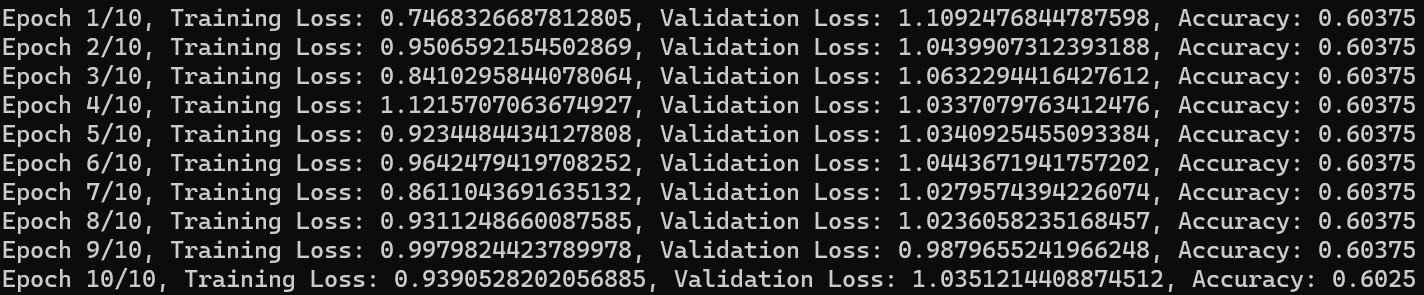
\includegraphics[width=0.5\linewidth]{融合实验结果.png}
    % \caption{Enter Caption}
    \label{fig:enter-label}
\end{figure}
但是有一个比较反常的现象,就是无论损失函数的值如何变化,模型的准确率从第一个epoch开始就稳定在$60.375\%$,没有再上升。我试着增加了卷积层的层数,并把ReLU函数更换为tanh、ELU等激活函数,但仍然没能解决这个问题,便只能作罢。我还试着把学习率跳到很小$1e-307$再训练模型,这时每一个epoch的验证准确率就会稳定在$10\%$到$20\%$这样一个比较低的水准。所以我推测,可能模型在训练完第一个epoch的时候就达到了损失函数的最优值点。我还打印出了模型在验证集上的预测结果,发现里面几乎全是positive。这可能还是由于模型还是比较简单。而且,训练集中positive的样本的数量也占到了大多数,所以模型也很难学习到neutral和negative样本的足够知识。
\subsubsection{消融实验结果}
消融实验就是分别只输入文本或图像数据,查看模型的表现。如果只输入图像,那就把文本模型的输出全部置为零,反之亦然:
\begin{lstlisting}
        if mode == 1:      #仅输入文本
            img_out *= 0
        elif mode == 2:    #仅输入图像
            txt_out *= 0
\end{lstlisting}
我们得到的结果如下:
\begin{figure}[h]
    \centering
    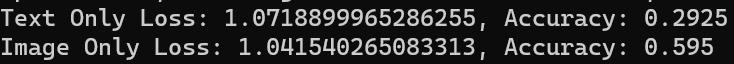
\includegraphics[width=0.5\linewidth]{消融实验结果.png}
    \label{fig:enter-label}
\end{figure}
这是一个耐人寻味的结果,只输入图像就能得到与融合实验差不多的准确率,而只输入文本,模型表现就会差很多。看来在融合实验中,也是图像起了主要作用。
\section{总结}
本次实验中,我们综合运用计算机视觉和自然语言处理的知识,通过图像、语言等不同形态的数据分析当事人的情感,更加深入地体会了人工智能的强大。

\end{document}